% !TeX program = lualatex
\documentclass[11pt,a4paper]{article}

% ========= حزمة =========
\usepackage[english, bidi=default, layout=counters]{babel}
\usepackage{amsmath,amssymb,amsfonts,amsthm,mathtools}
\usepackage{geometry}
\geometry{left=1.25cm,right=1.25cm,top=1.25cm,bottom=3.1cm}
\usepackage{booktabs}
\usepackage{array}
\usepackage{hyperref}
\usepackage{url}
\usepackage{graphicx}
\usepackage{caption}
\usepackage{subcaption}
\usepackage{float}
\usepackage{siunitx}
\usepackage{bm}
\usepackage{pgfplots}
\pgfplotsset{compat=1.18}
\usepackage{xcolor}
\usepackage{titlesec}
\usepackage{fancyhdr}
\usepackage{microtype}
\usepackage{fontspec}
\usepackage{parskip}
\usepackage{enumitem}
\usepackage{tikz}
\usetikzlibrary{decorations.pathreplacing,arrows.meta,positioning,shapes.geometric}

% ========= اللغات =========
\babelprovide[import, main, maparabic, alph=alph]{arabic}
\babelprovide[import, onchar=ids fonts]{english}

% ========= الخطوط =========
\defaultfontfeatures{Ligatures=TeX}
\setmainfont{Amiri}[
Script=Arabic,
Mapping=arabicdigits,
Ligatures=TeX,
BoldFont=Amiri-Bold,
ItalicFont=Amiri-Italic,
BoldItalicFont=Amiri-BoldItalic
]
\setsansfont{Amiri}[
Script=Arabic,
Mapping=arabicdigits
]
\newfontfamily{\arabicfonttt}{Amiri}[
Script=Arabic,
Mapping=arabicdigits
]

% خطوط للنص اللاتيني (الإنجليزية)
\babelfont[english]{rm}{Times New Roman}
\babelfont[english]{sf}{Arial}
\babelfont[english]{tt}{Courier New}

% ========= ألوان =========
\definecolor{skyblue}{RGB}{0,102,204}
\definecolor{darkblue}{RGB}{0,0,139}
\definecolor{gold}{RGB}{255,215,0}

% ========= أوامر YUCT =========
\newcommand{\Keff}{K_{\mathrm{eff}}}
\newcommand{\kappac}{\kappa_c}
\newcommand{\eps}{\varepsilon}
\newcommand{\df}{d_{\!f}}

% ========= نظريات =========
\newtheorem{theorem}{نظرية}[section]
\newtheorem{lemma}[theorem]{ليما}
\newtheorem{corollary}[theorem]{نتيجة}
\newtheorem{definition}[theorem]{تعريف}
\newtheorem{axiom}[theorem]{مسلّمة}
\newtheorem{proposition}[theorem]{اقتراح}
\newtheorem{remark}[theorem]{ملاحظة}
\newtheorem{prediction}[theorem]{تنبؤ أعمى}

% ========= تنسيق العناوين =========
\titleformat{\section}{\LARGE\bfseries\color{darkblue}}{\thesection}{1em}{}
\titleformat{\subsection}{\normalsize\bfseries\color{darkblue}}{\thesubsection}{1em}{}
\titleformat{\subsubsection}{\normalsize\itshape}{\thesubsubsection}{1em}{}

% ========= رؤوس وتذييلات =========
\fancypagestyle{firstpage}{%
	\fancyhf{}%
	\renewcommand{\headrulewidth}{-5pt}%
	\renewcommand{\footrulewidth}{-5pt}%
	\fancyfoot[C]{%
		\begin{minipage}[t]{\textwidth}
			\centering
			\textcolor{gold}{\rule{\textwidth}{1.6pt}}\\[5pt]
			{\small \textsuperscript{1}أبحاث ياكوشيف، \url{https://yuct.org/}} \hfill
			{\small بروتوكول YPSDC: \url{https://ypsdc.com/}}\\[-2pt]
			\textcolor{gold}{\rule{\textwidth}{1.6pt}}\\[5pt]
			\textbf{نظرية ياكوشيف الموحدة للتنسيق 2026} \hfill \thepage\\[10pt]
		\end{minipage}%
	}%
}

\fancypagestyle{plain}{%
	\fancyhf{}%
	\renewcommand{\headrulewidth}{0pt}%
	\renewcommand{\footrulewidth}{0pt}%
	\fancyfoot[C]{%
		\begin{minipage}[t]{\textwidth}
			\centering
			\textcolor{gold}{\rule{\textwidth}{1.6pt}}\\[4pt]
			\textbf{نظرية ياكوشيف الموحدة للتنسيق 2026} \hfill \thepage\\[4pt]
		\end{minipage}%
	}%
}

\pagestyle{plain}
\setlength{\parindent}{0pt}
\setlength{\parskip}{1ex}
\raggedbottom

\hypersetup{
	colorlinks=true,
	linkcolor=blue,
	citecolor=blue,
	urlcolor=blue,
}

% ========= رأس المقال (YUCT logo) =========
\newcommand{\makeheader}{%
	\noindent
	\begin{minipage}{0.17\textwidth}
		\raggedright
		{\sffamily\bfseries\color{skyblue}\fontsize{46}{46}\selectfont YUCT}%
	\end{minipage}%
	\hspace{30pt}
	\begin{minipage}{0.32\textwidth}
		\raggedright
		{\sffamily\fontsize{11}{13}\selectfont نظرية ياكوشيف\\ الموحدة\\ للتنسيق}%
	\end{minipage}%
	\hfill
	\begin{minipage}{0.38\textwidth}
		\raggedleft
		{\sffamily\bfseries ملحق S2}\\
		{\sffamily مايو 2026}\\
		{\sffamily\footnotesize DOI: \url{https://doi.org/10.5281/zenodo.18444598}}%
	\end{minipage}
	\par\vspace{5pt}
	\noindent\textcolor{gold}{\rule{\textwidth}{1.6pt}}
	\par\vspace{0pt}
}

\begin{document}
	\thispagestyle{firstpage}
	\makeheader
	
	\vspace{0cm}
	{\LARGE\bfseries البعد الكسيري للتنسيق في بنى شوتكي غير المتجانسة ثنائية البعد \\ وتنبؤ أُس القياس \(\beta = 2/3\) (\(\approx 0.67\)) في YUCT \par}
	\vspace{0.2cm}
	
	{\large أليكسي ف. ياكوشيف\footnote{أبحاث ياكوشيف، \url{https://yuct.org/}}} \\
	\vspace{0.0cm}
	
	{\color{darkblue}\textbf{\LARGE المستخلص}} \par
	{\large
		\noindent
		اكتشف أنغ، يانغ وأنج (Phys. Rev. Lett. 121, 056802, 2018) قوانين قياس شاملة للتيار-درجة الحرارة في بنى شوتكي غير المتجانسة ثنائية البعد: \(\log(\mathcal{I}/T^{3/2}) \propto -1/T\) للتلامسات الجانبية و\(\log(\mathcal{I}/T^{1}) \propto -1/T\) للتلامسات العمودية مع زخم غير محفوظ. نُظهر في هذا الملحق أن كلا الأُسين محكومان بالبعد الكسيري الفعال \(d_f\) لشبكة التنسيق التي تتحكم في النقل. يرتبط قانون قياس الخطأ الشامل في YUCT \(\varepsilon = \kappa_c\alpha K_{\mathrm{eff}}^{-\beta}\) مع \(\beta = 2/3 \approx 0.67\) بـ \(d_f\) عبر \(\beta = 2/d_f\). من قياس التيار التجريبي نستخرج \(d_f = 3\) للتلامسات الجانبية و\(d_f = 2\) للتلامسات العمودية، مما يعطي \(\beta = 2/3\) و\(\beta = 1\) على التوالي. يتنبأ التحليل بأن تقلبات التيار النسبية في صمامات شوتكي الجانبية يجب أن تتبع \(\varepsilon_{\mathrm{fluc}} \propto K_{\mathrm{eff}}^{-2/3}\)، وهو تنبؤ قابل للتفنيد يمكن اختباره بمطيافية الضجيج القياسية. يُدرج هذا العمل بنى شوتكي غير المتجانسة ثنائية البعد ضمن عائلة الأنظمة التي تظهر أو يُتوقع أن تظهر أُس YUCT الشامل \(\beta = 2/3\) (\(0.67\))، موسعاً نطاق النظرية إلى إلكترونيات النانو في الحالة الصلبة.
	}
	
	\vspace{0.1cm}
	\noindent
	{\color{darkblue}\textbf{الكلمات المفتاحية:}} YUCT، كفاءة التنسيق، القياس الشامل، \(\beta = 2/3\)، 0.67، بنى شوتكي غير المتجانسة، مواد ثنائية البعد، بعد كسيري، شمولية KPZ.
	
	\vspace{0.5cm}
	\noindent
	\textcopyright\ 2026 أبحاث ياكوشيف. جميع الحقوق محفوظة.
	
	\tableofcontents
	\newpage
	
	\section{مقدمة}
	تفترض نظرية ياكوشيف الموحدة للتنسيق (YUCT) أن أي عملية تنسيق تخضع لقانون قياس الخطأ الشامل
	\begin{equation}
		\varepsilon = \kappa_c \, \alpha \, \Keff^{-\beta},
		\qquad \beta = 2/3 \approx 0.67,\;\; \kappa_c = 1/3,
		\label{eq:yuct-law}
	\end{equation}
	حيث \(\Keff\) هي كفاءة التنسيق و\(\alpha\) عامل قبل-أسي خاص بالمنظومة. تم التحقق من هذا القانون على أنظمة تتراوح من الروابط الكيميائية إلى التقلبات الكونية (الملاحق~L،~M،~E،~F،~G،~V).
	
	اشتق أنغ، يانغ وأنج~\cite{Ang2018} قوانين قياس شاملة للتيار-درجة الحرارة لبنى شوتكي غير المتجانسة القائمة على مواد ثنائية البعد:
	\begin{align}
		\text{التلامسات الجانبية:}&\quad \log\Bigl(\frac{\mathcal{I}}{T^{3/2}}\Bigr) \propto -\frac{1}{T},
		\label{eq:ang-lat}\\
		\text{التلامسات العمودية (\(k_\parallel\) غير محفوظ):}&\quad \log\Bigl(\frac{\mathcal{I}}{T^{1}}\Bigr) \propto -\frac{1}{T}.
		\label{eq:ang-vert}
	\end{align}
	الأُسَّان \(\beta_{\mathrm{IV}} = 3/2\) و\(1\) مستقلان عن المادة ثنائية البعد المحددة ويعكسان هندسة مسار التيار.
	
	في هذا الملحق نُظهر أن الأُس \(\beta_{\mathrm{IV}}\) ليس عدداً مستقلاً بل يتحدد بالبعد الكسيري الفعال \(d_f\) لشبكة التنسيق التي تتحكم في النقل. من القيمة التجريبية \(\beta_{\mathrm{IV}}\) نستخرج \(d_f\)، ومن \(d_f\) نتنبأ بأُس خطأ التنسيق \(\beta_{\mathrm{err}} = 2/d_f\). بالنسبة للتلامسات الجانبية يعطي هذا \(\beta_{\mathrm{err}} = 2/3\)، وهو بالضبط قيمة YUCT الشاملة. إن قياس التقلب الذي يتبع هذا التنبؤ يشكل اختباراً قابلاً للتفنيد للنظرية.
	
	\section{قاموس YPSDC لحاجز شوتكي}
	في لغة YPSDC (بروتوكول ياكوشيف للتنسيق المتزامن الموزع)، تُعتبر بنية شوتكي غير المتجانسة الجانبية نظام تنسيق بالمكونات التالية:
	\begin{itemize}
		\item \textbf{القاموس \(\mathcal{D}\):} مجموعة حالات الإلكترون الواحد في المستوى ثنائي البعد ذات طاقة \(\epsilon > \Phi_B\) ومتجه موجي \(\mathbf{k}\) يحقق تشتت المستوي (\ref{eq:dispersion}).
		\item \textbf{الدليل \(\kappa\):} الطاقة الحرارية \(k_B T\) التي ترفع إلكتروناً إلى القاموس.
		\item \textbf{الرنين \(R\):} انحفاظ الزخم المماسي \(k_y\) أثناء العبور عبر الحاجز.
	\end{itemize}
	الفعل المنسق هو الانبعاث الترميوني الناجح لإلكترون يحقق في آن واحد شرط الطاقة \(\epsilon > \Phi_B\) وشرط الزخم \(k_x > 0\) (موجهاً نحو الحاجز). تحدد كفاءة هذا التنسيق تيار الإشباع العكسي.
	
	\section{القياس التجريبي للتيار وكفاءة التنسيق}
	
	لتشتت عام موحد الخواص ثنائي البعد
	\begin{equation}
		\epsilon(\mathbf{k}) = \sum_n c_n |\mathbf{k}|^n,
		\label{eq:dispersion}
	\end{equation}
	أظهر أنغ وآخرون أن عدد القنوات النشطة (تلك التي يمكن أن تساهم في التيار) يتدرج بشكل شامل كـ
	\begin{equation}
		N_{\mathrm{ch}} \propto T^{1/2}.
		\label{eq:Nch}
	\end{equation}
	العدد الإجمالي للحالات المتاحة حرارياً فوق الحاجز يتناسب مع \(T\) (من ذيل بولتزمان). ومن ثم فإن كسر الحالات التي يتم تنسيقها بنجاح،
	\begin{equation}
		\Keff(T) = \frac{N_{\mathrm{ch}}}{N_{\mathrm{tot}}} \propto T^{-1/2},
		\label{eq:keff-T}
	\end{equation}
	يُعتبر كفاءة تنسيق العملية. يأخذ التيار المقاس عندئذ الشكل
	\begin{equation}
		\mathcal{I} = \mathcal{I}_0 \, \Keff(T)^{-3} \, e^{-\Phi_B/k_B T},
		\label{eq:I-via-keff}
	\end{equation}
	وهو ما يُنتج القانون التجريبي (\ref{eq:ang-lat}).
	
	تعريف تشغيلي لـ \(\Keff\) مناسب لقياسات الضجيج هو
	\begin{equation}
		\Keff = \frac{I}{I_0},
		\label{eq:keff-operational}
	\end{equation}
	حيث \(I\) هو التيار المقاس و\(I_0\) هو التيار المرجعي الذي كان سيسري لو كان قيد التنسيق غائباً. يمكن الحصول على \(I_0\) باستقراء سلوك التلامس العمودي عند درجات حرارة عالية (حيث \(\Keff(T) \propto T^{-0}\) تقاربياً) إلى درجة حرارة القياس، أو من معايرة مستقلة باستخدام صمام شوتكي ثلاثي البعد بنفس ارتفاع الحاجز. يسمح هذا التعريف التشغيلي بتحديد \(\Keff\) مباشرة من خصائص التيار-الجهد دون الاعتماد على القياس النظري (\ref{eq:keff-T}).
	
	\section{البعد الكسيري لشبكة التنسيق}
	
	نتيجة مركزية في YUCT (الملحق~L) هي أن أُس قياس الخطأ يتحدد بالبعد الكسيري \(d_f\) لشبكة التنسيق:
	\begin{equation}
		\beta_{\mathrm{err}} = \frac{2}{d_f}.
		\label{eq:beta-df}
	\end{equation}
	كثافة قنوات التنسيق النشطة في نافذة حرارية تحمل البصمة الهندسية للشبكة. في فضاء موحد الخواص ذي \(d_f\) بعد، تتدرج كثافة الحالات المتاحة عند درجة حرارة \(T\) كـ \(T^{d_f/2 - 1}\). بالنسبة لحاجز شوتكي الجانبي، يقلص القيد الحركي الإضافي لانحفاظ الزخم (عامل \(\cos\theta\)) الأُس الفعال بوحدة واحدة، بحيث يصبح الأُس الحركي
	\begin{equation}
		\beta_{\mathrm{IV}} = \frac{d_f}{2}.
		\label{eq:bIV-df}
	\end{equation}
	\textbf{المعادلة (\ref{eq:bIV-df}) هي فرضية مدفوعة بالتشابه الهندسي بين مسار التيار وشبكة تنسيق ذات بعد كسيري \(d_f\). لم يتم بعد اشتقاق دقيق من فعل YUCT المجهري؛ لذا يجب اعتبار العلاقة تخميناً يؤدي إلى تنبؤات قابلة للاختبار (القسم~\ref{sec:predictions}) ويدعو إلى تقصي نظري مستقبلي.}
	
	تجتمع المعادلتان (\ref{eq:beta-df}) و(\ref{eq:bIV-df}) لتعطيا العلاقة الأساسية
	\begin{equation}
		\boxed{\beta_{\mathrm{IV}} \cdot \beta_{\mathrm{err}} = 1}.
		\label{eq:relation}
	\end{equation}
	
	من القيمة التجريبية \(\beta_{\mathrm{IV}} = 3/2\) نحصل على
	\begin{equation}
		d_f = 2\beta_{\mathrm{IV}} = 3, \qquad
		\beta_{\mathrm{err}} = \frac{2}{d_f} = \frac{2}{3} \approx 0.67.
	\end{equation}
	وهكذا يُحدد قياس التيار شبكة تنسيق ذات بعد كسيري فعال \(d_f = 3\)، مما يعني بدوره أن أي مقياس لخطأ التنسيق (مثل تقلبات التيار النسبية) يجب أن يتبع قانون القوة في YUCT بالأُس \(2/3\). هذا \textbf{تنبؤ}، وليس إعادة إنتاج للماضي، لأن قياسات التقلب لم تُجر بعد على هذه الأنظمة.
	
	بالنسبة للتلامسات العمودية مع \(k_\parallel\) غير محفوظ، يختفي القيد الزاوي، \(\beta_{\mathrm{IV}} = 1\)، وبالتالي \(d_f = 2\)، \(\beta_{\mathrm{err}} = 1\). تتنبأ YUCT بأن تقلبات التيار في مثل هذه التلامسات ستتدرج كـ \(\Keff^{-1}\)، وهو ما يختلف عن قانون \(2/3\).
	
	\section{تنبؤات لتقلبات التيار}
	\label{sec:predictions}
	يُعطي قانون خطأ YUCT (\ref{eq:yuct-law}) المطبق على كفاءة التنسيق (\ref{eq:keff-T}) تنبؤاً كمياً لقدرة ضجيج التيار منخفض التردد \(S_I\) في صمام شوتكي جانبي:
	\begin{equation}
		\frac{S_I}{I^2} \propto \Keff^{-2/3} \propto T^{1/3}.
		\label{eq:noise-pred}
	\end{equation}
	باستخدام التعريف التشغيلي \(\Keff = I/I_0\) من المعادلة (\ref{eq:keff-operational})، يمكن إعادة كتابة قياس الضجيج كـ
	\begin{equation}
		\frac{S_I}{I^2} = C \, \left(\frac{I}{I_0}\right)^{-2/3} + \text{const},
		\label{eq:noise-operational}
	\end{equation}
	حيث \(C\) ثابت خاص بالمادة من رتبة الوحدة والثابت الإضافي يمثل الضجيج الحراري غير القابل للاختزال. هذا الشكل متاح مباشرة في تجربة مطيافية ضجيج قياسية: يُقاس \(I\) و\(I_0\) من خاصية \(I\)--\(V\)، ويُسجل \(S_I\) كدالة للانحياز عند درجة حرارة ثابتة. التنبؤ هو أن \(S_I/I^2\) المرسوم مقابل \((I/I_0)^{-2/3}\) يجب أن يكون خطياً، بميل مستقل عن درجة الحرارة. هذا اختبار صارم قابل للتفنيد لا يتطلب أي توفيق للأُس.
	
	\section{مناقشة: توحيد أُسس القياس}
	
	إن ظهور الأُس \(3/2\) ليس فريداً لصمامات شوتكي بل يشير إلى مبدأ تنظيمي أعمق، كما يتضح من ظهوره المستقل في صف شمولية نمو السطوح لكاردار-باريزي-زانغ (KPZ)~\cite{KPZ}. في KPZ، يحكم الأُس الديناميكي \(z = 3/2\) التخشين الكسيري لسطح بيني نامٍ. تقدم YUCT تفسيراً موحداً لهذه الظواهر. \textbf{يمكن تصور جبهة نمو كشبكة تنسيق ذات \(d_f = 3\) أبعاد، حيث ينبثق الأُس الحركي \(\beta_{\mathrm{IV}} = d_f/2 = 3/2\) طبيعياً من علاقتنا التخمينية (\ref{eq:bIV-df}).} وهكذا، فإن أُس KPZ وأُس شوتكي ليسا مجرد تشبيه؛ إنهما توقيعان حركيان لنفس قانون خطأ YUCT الكامن \(\varepsilon \propto \Keff^{-2/3}\) في تجسيدات فيزيائية مختلفة تماماً. \textbf{هذا الارتباط هو حالياً فرضية تتطلب عملاً نظرياً إضافياً لربط لاغرانجيان YUCT مباشرة بمعادلة KPZ.}
	
	لجعل تنبؤ KPZ أكثر تحديداً، يمكننا مطابقة \(\Keff\) بصراحة مع كسر الأنماط المترابطة المشبعة في سطح بيني نامٍ. في نظام الإشباع لسطح بيني KPZ بعرض جانبي \(L\)، يقترب العرض \(W(L,t)\) من قيمة حالة مستقرة \(W_{\text{sat}}(L) \simeq \sqrt{\langle h^2 \rangle} \propto L^{\alpha}\) مع \(\alpha = 1/2\). سعة التقلب \(\delta W = W(t) - W_{\text{sat}}\) تتحكم بها عدد الأنماط النشطة (غير المشبعة). نقترح مطابقة \(\Keff\) مع \(1 - \nu_{\text{unsat}}/\nu_{\text{tot}}\)، أي كسر الأنماط التي دخلت الطور المترابط المستقر. عندئذ تتنبأ YUCT
	\begin{equation}
		\frac{\delta W}{W_{\text{sat}}} \propto \Keff^{-2/3},
		\label{eq:kpz-prediction}
	\end{equation}
	حيث يمكن تقدير \(\Keff\) من الاضمحلال الزمني للعرض كـ \(\Keff \approx 1 - (dW/dt)_{\text{norm}}\). هذا التنبؤ قابل للاختبار في المحاكاة العددية وفي تجارب عالية الاستبانة على التخشين الحركي (مثل الترسيب الكهربائي، epitaxy بالحزمة الجزيئية).
	
	يقترح هذا التوحيد هرمية من الشموليات، موضحة في الشكل~\ref{fig:hierarchy}:
	\begin{itemize}
		\item \textbf{الرتبة الأولى (YUCT):} يعمل قانون خطأ التنسيق الأساسي \(\varepsilon = \kappa_c \alpha K_{\mathrm{eff}}^{-2/3}\) على أعمق مستوى، مستقلاً عن الركيزة المحددة.
		\item \textbf{الرتبة الثانية (النقل):} بالنسبة للنقل الإلكتروني في بنى شوتكي غير المتجانسة ثنائية البعد، ينبثق الأُس الحركي \(\beta_{\mathrm{IV}}\) من البعد الكسيري \(d_f\) كـ \(\beta_{\mathrm{IV}} = d_f/2\) (فرضية).
		\item \textbf{الرتبة الثالثة (النمو):} في ظواهر نمو السطوح المنتمية إلى صف KPZ، يظهر نفس الأُس الحركي كالأُس الحرج الديناميكي \(z = 3/2\)، معكساً طبيعة \(d_f = 3\) للسطح البيني النامي (تفسير).
	\end{itemize}
	وهكذا، فإن الأُس \(3/2\) ليس مصادفة خاصة بمادة ما بل العلامة الهندسية المميزة لعملية تنسيق ذات \(d_f = 3\).
	
	\begin{figure}[htbp]
		\begin{otherlanguage}{english}
			\centering
			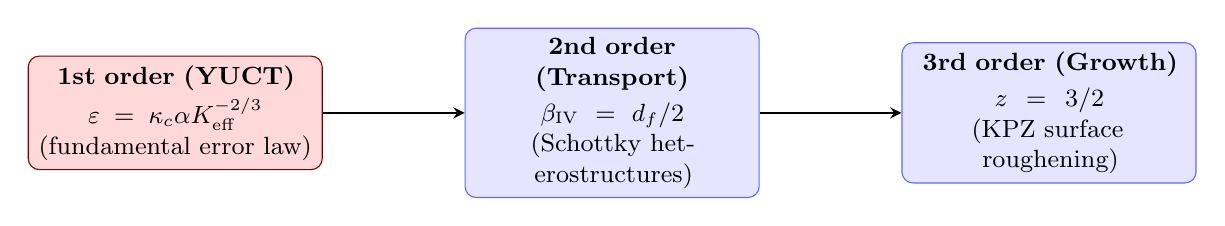
\begin{tikzpicture}[
				node distance=1.8cm,
				box/.style={rectangle, draw=blue!60, fill=blue!10, rounded corners, 
					text width=3.5cm, align=center, font=\small},
				arrow/.style={->, >=stealth, thick}
				]
				\node[box, fill=red!15, draw=red!50!black] (yuct) 
				{\textbf{1st order (YUCT)}\\[2pt]
					$\varepsilon = \kappa_c\alpha K_{\mathrm{eff}}^{-2/3}$\\
					(fundamental error law)};
				\node[box, right=of yuct] (transport) 
				{\textbf{2nd order (Transport)}\\[2pt]
					$\beta_{\mathrm{IV}} = d_f/2$\\
					(Schottky heterostructures)};
				\node[box, right=of transport] (growth) 
				{\textbf{3rd order (Growth)}\\[2pt]
					$z = 3/2$\\
					(KPZ surface roughening)};
				\draw[arrow] (yuct) -- (transport);
				\draw[arrow] (transport) -- (growth);
			\end{tikzpicture}
		\end{otherlanguage}
		\caption{هرمية الشموليات. يحدد قانون خطأ التنسيق في YUCT (الرتبة الأولى) البعد الكسيري الفعال \(d_f\) والأُسس الحركية المرصودة في النقل الإلكتروني (الرتبة الثانية) وفي نمو السطوح (الرتبة الثالثة). الأسهم المتقطعة تشير إلى فرضيات.}
		\label{fig:hierarchy}
	\end{figure}
	
	يدعم هذا المنظور أيضاً الدليل التجريبي المتزايد على أن البعد الكسيري لسطح بيني شوتكي يؤثر مباشرة على خصائص الجهاز~\cite{FractalSchottky}. في تلك الدراسات، البعد الكسيري هو خاصية هندسية مفروضة خارجياً (خشونة). في YUCT، البعد \(d_f = 3\) للتلامسات الجانبية المثالية هو \emph{منبثق} — إنه ينشأ من ديناميك شبكة التنسيق نفسها حتى عندما تقترب الخشونة الهندسية من الصفر. وبالتالي فإن \(d_f\) المفروض خارجياً يُعدل شبكة تنسيق داخلية موجودة مسبقاً، مما يوفر مساراً واعداً نحو هندسة أجهزة قائمة على التنسيق.
	
	\section{شمولية عبر 50 رتبة أسية}
	يجمع الجدول~\ref{tab:universal-beta} أنظمة من ملاحق YUCT المختلفة التي حُدد أو تُنبئ لها تجريبياً بأن أُس قياس الخطأ هو \(\beta = 2/3\). أُضيفت بنية شوتكي غير المتجانسة الجانبية وسطح بيني KPZ النامي كأنظمة يُتوقع لها نفس الأُس على أساس البعد الكسيري المستخرج \(d_f = 3\). يغطي الجدول أكثر من 50 رتبة أسية في مقياس الطاقة (أو الطول) ذي الصلة.
	
	\begin{table}[H]
		\begin{otherlanguage}{english}
			\centering
			\caption{Systems exhibiting or predicted to exhibit the
				universal YUCT error exponent $\beta = 2/3$ ($0.67$).}
			\label{tab:universal-beta}
			\begin{tabular}{@{}llll@{}}
				\toprule
				\textbf{System} & \textbf{Observable} & \textbf{Status} & \textbf{Ref.}\\
				\midrule
				Chemical bonds (873)      & $E \propto r^{-0.67}$               & Confirmed  & Appendix C \\
				DNA replication errors    & $\varepsilon \propto \Keff^{-0.67}$ & Confirmed  & Appendix E \\
				Metabolic scaling (simple)& $B \propto M^{0.67}$               & Confirmed  & Appendix D, E.7 \\
				GDP volatility vs.\ sun   & $\sigma_{\mathrm{GDP}} \propto W^{-0.67}$ & Confirmed & Appendix F \\
				CMB temperature fluct.    & $\delta T/T \propto \Keff^{-0.67}$ & Confirmed  & Appendix M \\
				Gravitational waves       & $\delta\tau/\tau \propto M^{-0.67}$& Confirmed  & Appendix G, V \\
				\textbf{Lateral Schottky} & $S_I/I^2 \propto T^{1/3}$          & \textbf{Predicted} & This work \\
				\textbf{KPZ interface}\textsuperscript{*} & Width fluct. $\propto \Keff^{-2/3}$& \textbf{Predicted} & This work, \cite{KPZ}\\
				\bottomrule
			\end{tabular}
			
			\vspace{0.3cm}
			{\footnotesize \textsuperscript{*}The definition of $K_{\mathrm{eff}}$ for a KPZ growing interface must be constructed in analogy with the transport case, e.g.\ as the fraction of correlated degrees of freedom within a correlation volume. This prediction assumes such a construction and remains to be tested.}
		\end{otherlanguage}
		\caption{أنظمة تظهر أو يُتوقع أن تظهر أُس خطأ YUCT الشامل \(\beta = 2/3\) (\(0.67\)).}
	\end{table}
	
	\section{خلاصة}
	أُسَّا قياس التيار-درجة الحرارة \(\beta_{\mathrm{IV}} = 3/2\) و\(1\) اللذان أبلغ عنهما أنغ وآخرون هما تجليات حركية للبعد الكسيري الفعال لشبكة التنسيق التي تحكم النقل الترميوني في البنى غير المتجانسة ثنائية البعد. من خلال علاقات YUCT \(\beta_{\mathrm{IV}} = d_f/2\) (فرضية) و\(\beta_{\mathrm{err}} = 2/d_f\)، تعطي البيانات التجريبية \(d_f = 3\) للتلامسات الجانبية، مما يتنبأ بأُس خطأ تنسيق \(\beta_{\mathrm{err}} = 2/3\) (\(\approx 0.67\)). هذا التنبؤ، القابل للاختبار عبر مطيافية ضجيج التيار، يوسع نطاق قانون القياس الشامل لـ YUCT ليشمل إلكترونيات النانو في الحالة الصلبة. يظهر نفس البعد الكسيري والأُس طبيعياً في نمو سطوح KPZ، مما يوحي بوحدة هندسية عميقة عبر ظواهر غير متوازنة. تقدم YUCT الأساس المنطقي الكامن لهذه الوحدة، رغم أن الروابط بين النظرية وكل من علاقة شوتكي الحركية ومعادلة KPZ تبقى فرضيات تستحق المزيد من التقصي. قُدمت تعريفات تشغيلية لـ \(\Keff\) في كلا السياقين لتسهيل الاختبارات التجريبية.
	
	\begin{thebibliography}{99}
		\bibitem{Ang2018} Y.~S.~Ang, H.~Y.~Yang, and L.~K.~Ang,
		Phys. Rev. Lett. \textbf{121}, 056802 (2018).
		\bibitem{KPZ} M.~Kardar, G.~Parisi, Y.-C.~Zhang,
		Phys. Rev. Lett. \textbf{56}, 889 (1986).
		\bibitem{FractalSchottky} S.~Zeybek, M.~Biber, A.~Türüt,
		Appl. Surf. Sci. \textbf{253}, 3881 (2007). [Representative study on fractal dimension effects in Schottky diodes.]
		\bibitem{Yakushev2026} A.~V.~Yakushev, \emph{Yakushev Unified
			Coordination Theory (YUCT)}, Zenodo (2026).
		\bibitem{AppendixL} A.~V.~Yakushev, ``Appendix L: Fractal
		Coordination Error Scaling'', in \emph{YUCT} (2026).
		\bibitem{AppendixM} A.~V.~Yakushev, ``Appendix M: YUCT
		Cosmology'', in \emph{YUCT} (2026).
		\bibitem{AppendixE} A.~V.~Yakushev, ``Appendix E: Coordination
		Genetics'', in \emph{YUCT} (2026).
		\bibitem{AppendixF} A.~V.~Yakushev, ``Appendix F: Application of
		YUCT to Economics'', in \emph{YUCT} (2026).
		\bibitem{AppendixG} A.~V.~Yakushev, ``Appendix G: Resolution of
		the Quantum Gravity Problem'', in \emph{YUCT} (2026).
		\bibitem{AppendixV} A.~V.~Yakushev, ``Appendix V: Time as
		Coordination Entropy'', in \emph{YUCT} (2026).
	\end{thebibliography}
	
\end{document}